
\hypertarget{working_hotkeys}{}
\section{Hotkeys (operational system)}
\index{hotkeys}

\begin{figure}[H]
  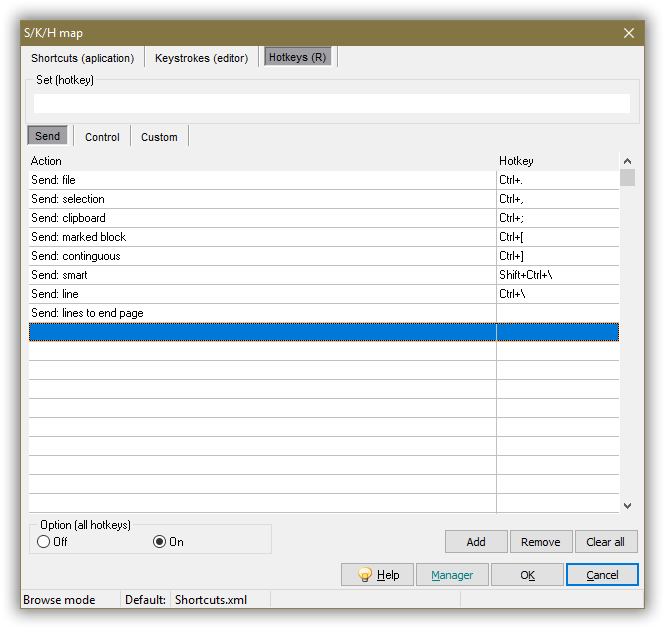
\includegraphics[scale=0.36]{./res/hotkeys_send.png}
  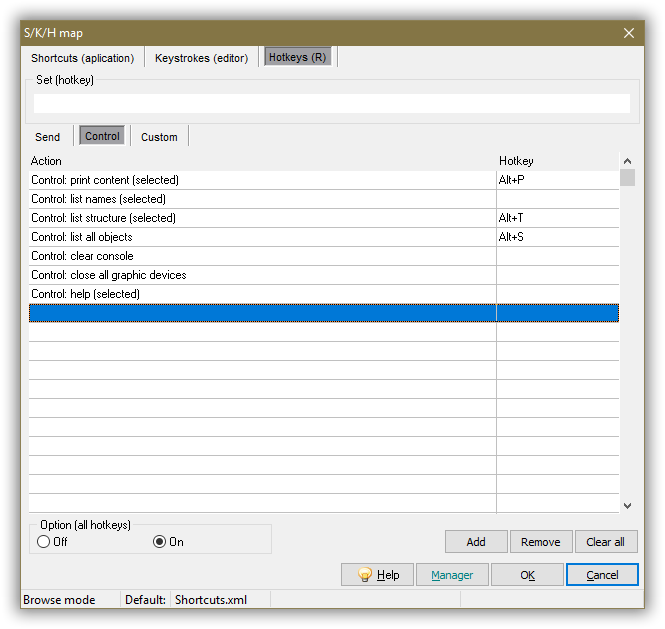
\includegraphics[scale=0.36]{./res/hotkeys_control.png}
  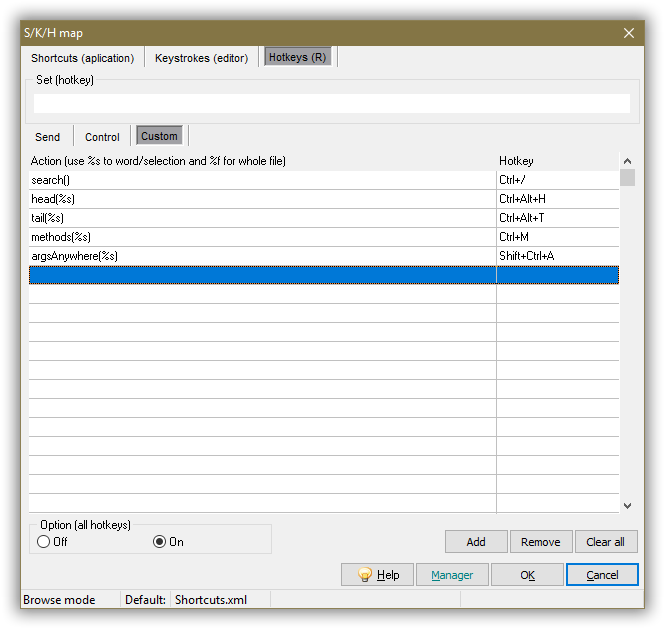
\includegraphics[scale=0.36]{./res/hotkeys_custom.png}
  \caption{Hotkeys.}
  \label{fig:hotkeys}
\end{figure}

The \textit{Hotkeys (operational system)}
(Figure \ref{fig:hotkeys})
allow setting the hotkeys
related to the operational system. The difference between those hotkeys and
\textit{Shortcuts customization} is that the latter works only with the
focus in Tinn-R, whereas the hotkeys work with the focus anywhere.

The interface is self-explanatory. Basically you first make a choice from
the \textit{R/Hotkeys (operational system)} and set the desired Hotkey.

The set of hotkeys will perform actions only if the option \textit{Active}
is checked. The objective of these options (\textit{Inactive} and
\textit{Active}) is to avoid conflict with others applications allowing
to enable/disable the set of hotkeys quickly and easily.

The \texttt{R/Hotkeys} interface was deeply reworked in the version 2.4.0.0 and it now has two tabs,
\texttt{Default} and \texttt{Custom}:

\begin{itemize}
\item \texttt{Default}: Contains the already traditional instructions of Tinn-R;
\item \texttt{Custom}: \textbf{Allows the user to customize any instructions} to be send to \RR{} interpreter (thanks to Philemon Lenherr for the suggestion). The instructions must be as follows:
 \begin{itemize}
 \item Simple: \texttt{search()}. The \RR{} interpreter will receive \texttt{$>$ search()};
 \item Replace word or small selection: \texttt{View(\%s, title='View of iris dataset')}.
   If the editor cursor is over the word \texttt{iris} or it is selected,
   the \RR{} interpreter will receive \texttt{$>$ View(iris, title='View of iris dataset')}
 \item Replace whole file: \texttt{source(\%f, echo=TRUE, verbose=TRUE)}.
   The \RR{} interpreter will receive \texttt{$>$ source(.trPaths[4], echo=TRUE, verbose=TRUE)}.
   All rules related to send file are preserved.
 \end{itemize}
\end{itemize}
